\begin{frame}{Les plongées \emph{techniques} pour le N1}
\begin{block}<only@1>{Ce qu'il faut viser}
\begin{itemize}
\item[\twemoji{penguin}] 4 plongées, limite\dots
\item[\twemoji{octopus}] 5 plongées, c'est mieux, 
\item[\twemoji{dolphin}] $\ge 6$ plongée, c'est cool.
%\item \twemoji{whale}, \twemoji{octopus}, \twemoji{fish}, \twemoji{tropical_fish}, \twemoji{blowfish}, \twemoji{penguin}, \twemoji{dolphin}, \twemoji{spouting whale}
\end{itemize}
\end{block}
\only<2>{%
\framesubtitle{Méjean}
\begin{minipage}{0.48\textwidth}
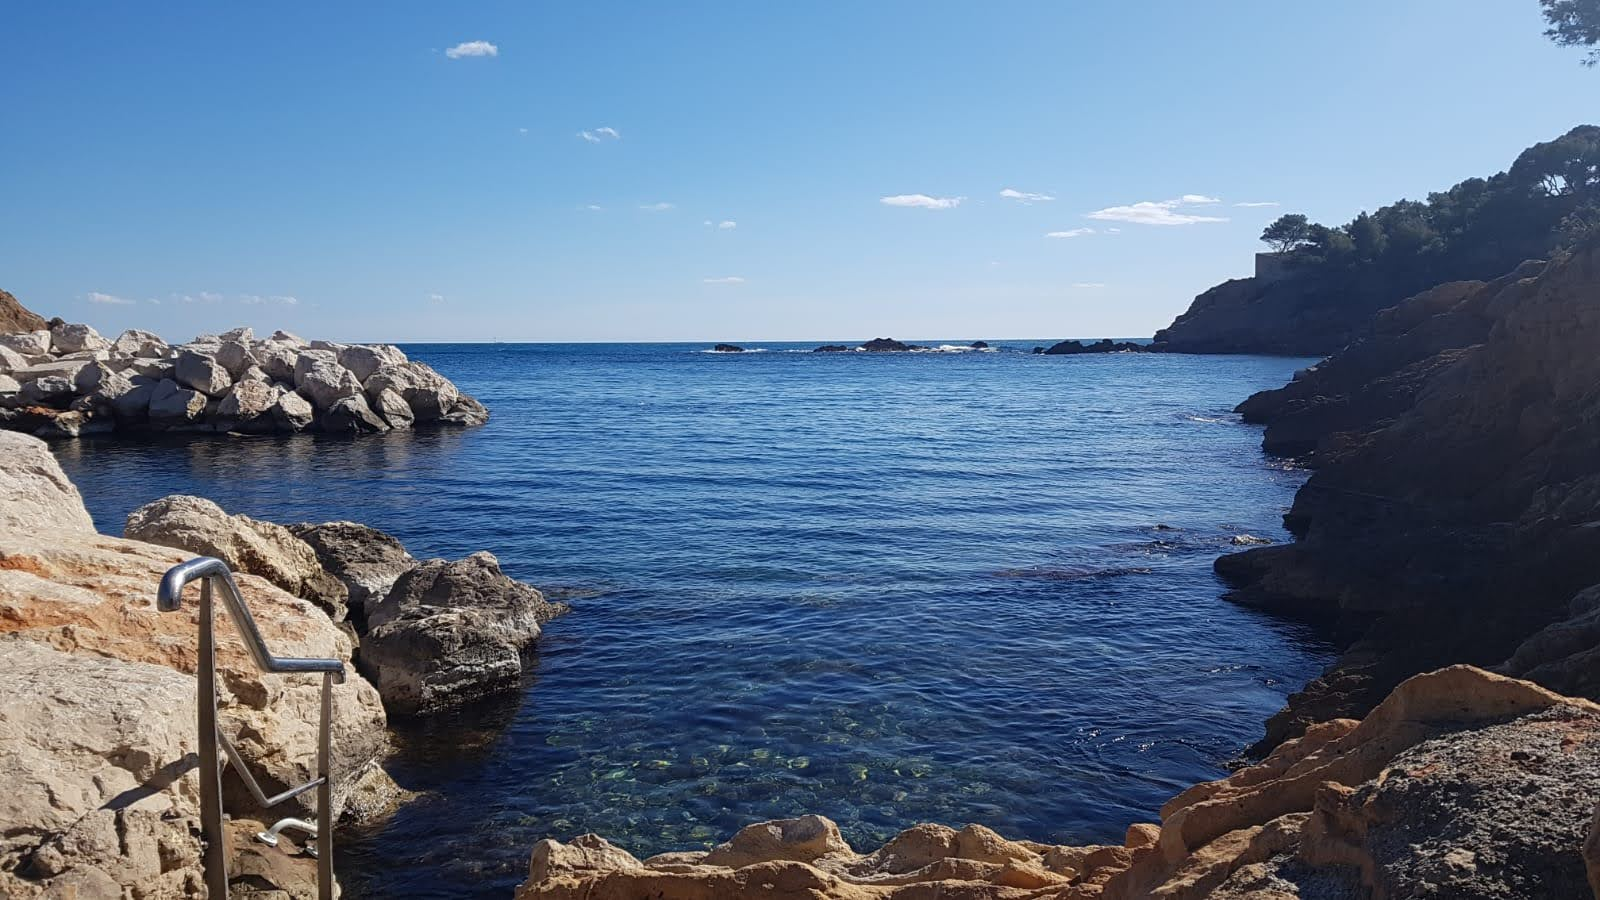
\includegraphics[width=\textwidth]{Mejean}
\end{minipage}\hfill
\begin{minipage}{0.48\textwidth}
\begin{exampleblock}{Idéal pour la mise à l'eau}
\begin{itemize}
\item départ du bord
\item protégé
\item peu profond
\end{itemize}
\end{exampleblock}
\end{minipage}
}%
\only<3>{%
\framesubtitle{Marseille}
\begin{minipage}{0.48\textwidth}
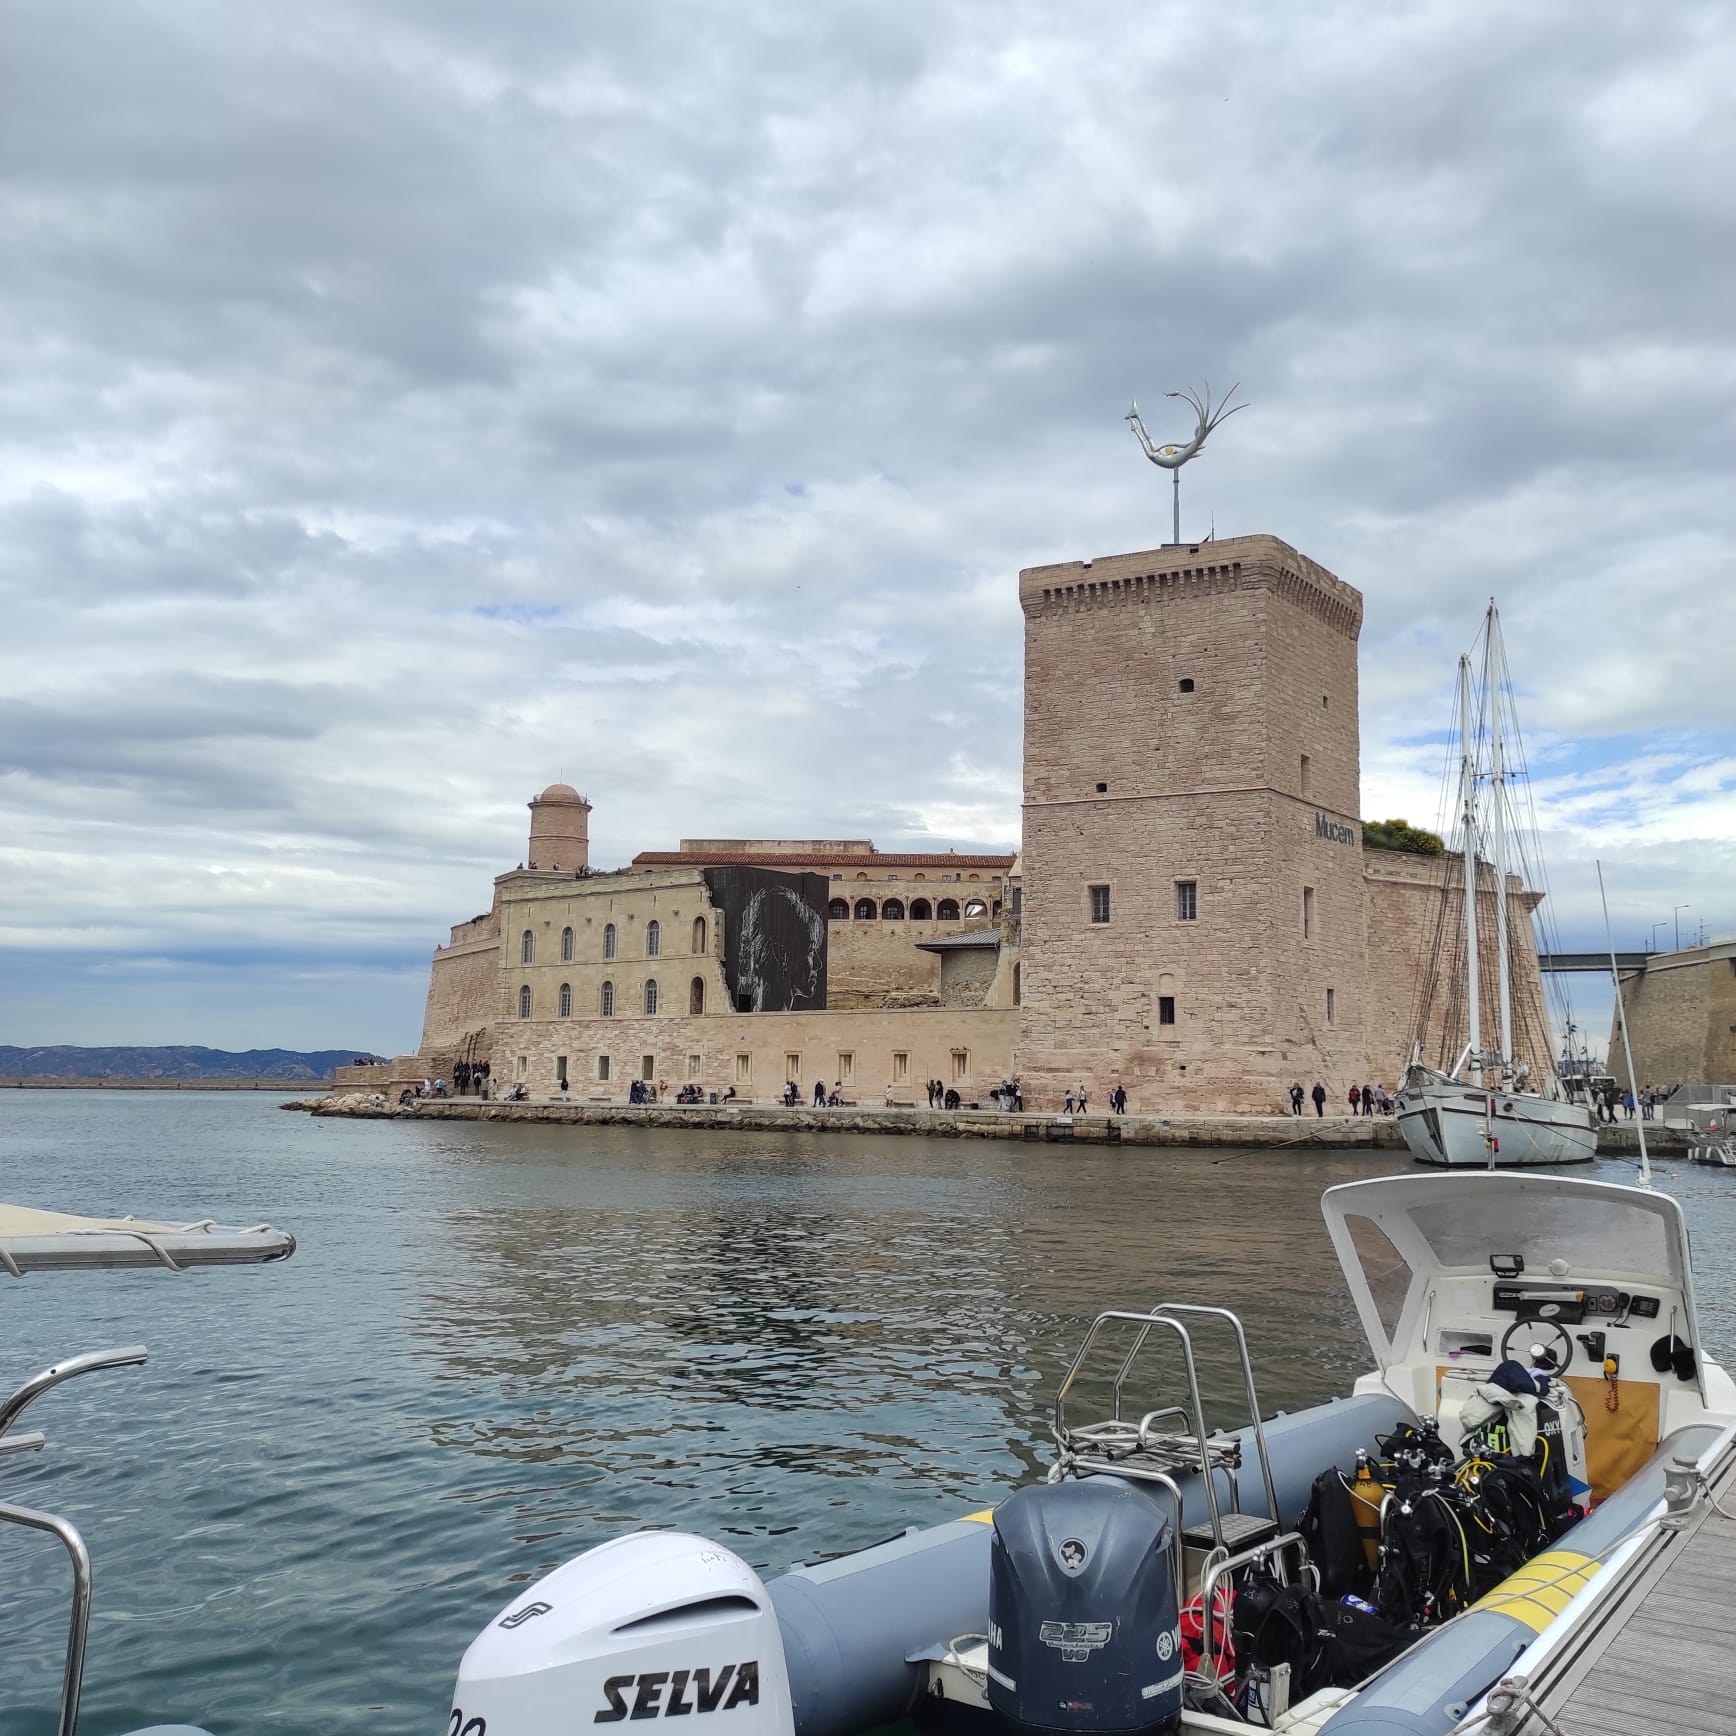
\includegraphics[width=\textwidth]{Marseille}
\end{minipage}\hfill
\begin{minipage}{0.48\textwidth}
\begin{exampleblock}{Idéal pour la suite}
\begin{itemize}
\item bonne visibilité
\item bascule arrière facile
\end{itemize}
\end{exampleblock}
\end{minipage}
}%
\begin{alertblock}<only@4>{Et donc\dots}
\huge Favoriser un maximum ces sorties pour valider le N1!
\end{alertblock}
\end{frame}

%
%\begin{frame}{S'incrire/payer}
%\centering%
%\includegraphics<1>[height=0.9\textheight]{inscription_formulaire}
%\includegraphics<2>[width=0.7\textwidth]{inscription_reservation}
%\end{frame}

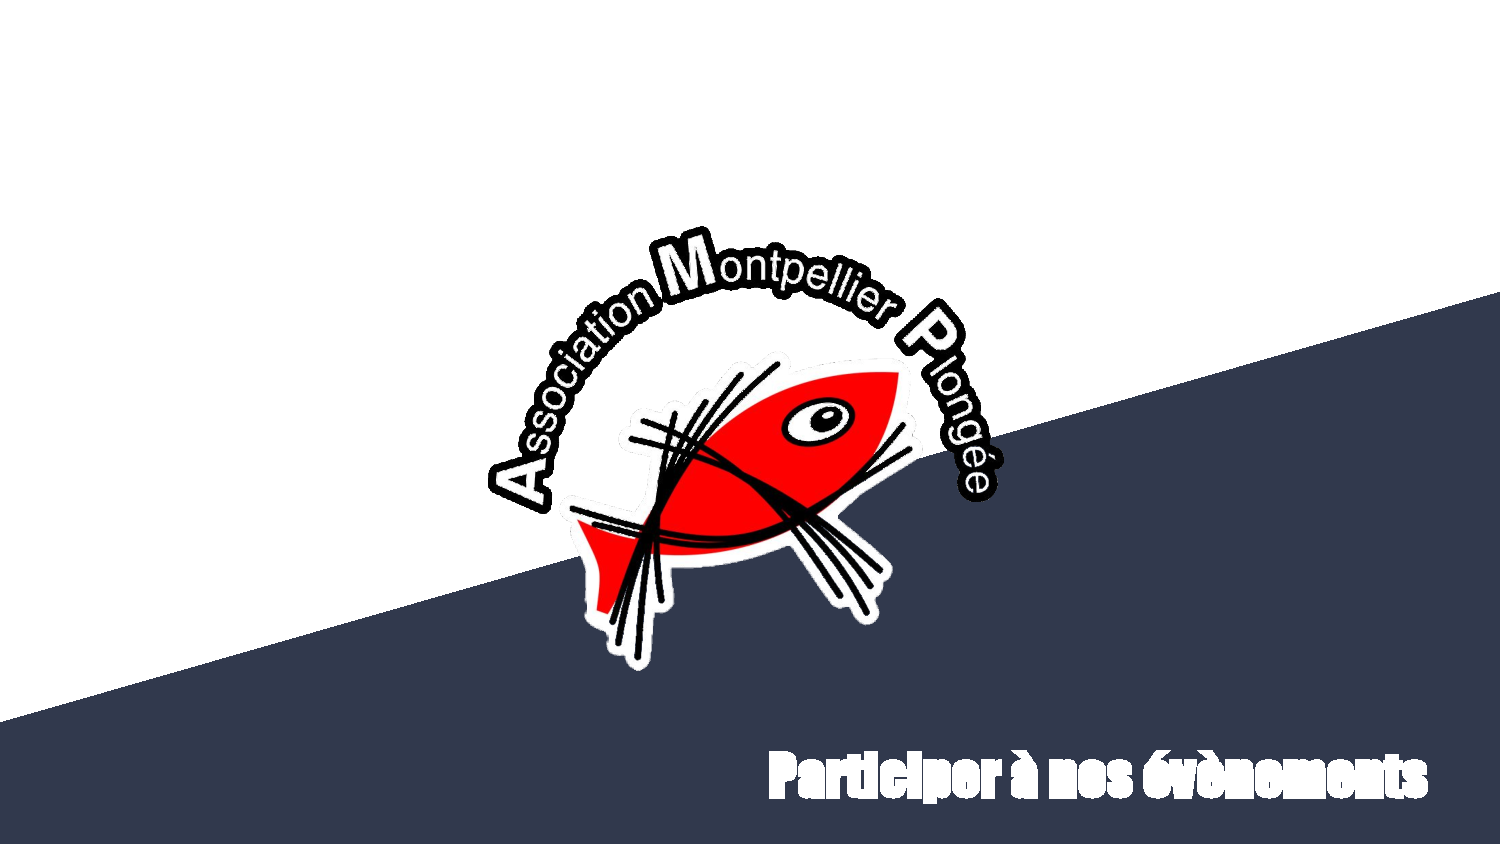
\includepdf[pages=-]{AMP-Participer_aux_evenements_juin_2025}

